%% Version 0.001 of Poly PhD thesis template.
%% Time-stamp: <2011-12-27 14:52:09 Boris Aronov>

\documentclass[letterpaper]{polythesis} 

%% This controls the sizes, spacing, and font of section headings.  It
%% does NOT control the layout of chapter header pages.  There are
%% many different styles possible.
\usepackage[medium]{titlesec}

% Allows box rotation.  Uncomment if you need it.
% \usepackage{rotate}

%% Using CMR fonts.  Add appropriate font commands if you want to
%% switch to something else.  Be warned that there are virtually zero
%% text/math font combinations available that work well in TeX.  It's
%% a standard TeX FAQ

\usepackage{calc}

%% Occasionally needed for weird footnote behavior  Do not use if you
%% have no footnotes in your thesis.
%\usepackage[bottom]{footmisc}

%% WARNING:  This will BREAK if your subfigure.sty is v2.0 or before!
\usepackage[subfigure]{ccaption}
\usepackage{subfigure}

%\usepackage{type1cm}
\usepackage{url, cite, graphicx, algorithmic, amsmath, amsfonts, amsthm}
\usepackage[chapter]{algorithm}

%% this is a customized package
%% Do NOT use unless you ABSOLUTELY have to.  Nesting sections that
%% deep is ridiculous.
% \usepackage{subsections}
% \setcounter{secnumdepth}{5}
% \setcounter{tocdepth}{5}

%% Abbreviations that you might need...
% \newcommand{\AA}{\mathcal{A}}
% \newcommand{\reals}{\mathbb{R}}
% ...

\newtheorem{condition}{Condition}[section]
\newtheorem{definition}{Definition}[section]
\newtheorem{theorem}{Theorem}[section]
\newtheorem{lemma}[theorem]{Lemma}
\newtheorem{cor}[theorem]{Corollary}
\newtheorem{corollary}[theorem]{Corollary}
\newtheorem{claim}[theorem]{Claim}
\newtheorem{fact}[theorem]{Fact}
\newtheorem{example}[section]{Example}
\newtheorem{note}{Note}[section]

%% Some trickery to be able to add stuff in before the first chapter.
\def\nonumchapter#1{%
    \chapter*{#1}
    \addcontentsline{toc}{chapter}{#1}}

\def\prefacesection#1{%
    \chapter*{#1}
    \addcontentsline{toc}{chapter}{#1}}

\def\afterpreface{\newpage
    \pagenumbering{arabic}
    \typeout{Thesis preface pages completed.}
    }

%% New operators if you need them.
% \DeclareMathOperator{\area}{area}

%% Uncomment if you need to see every file your document uses, with
%% all versions.
% \listfiles

\begin{document}

\frontmatter

\title{Fancy Research Results of World-Wide Importance}
\author{Generic M.\ Student}

\date{\today}

\pagenumbering{roman}

\maketitle

{\setstretch{2}
% $Id: title.tex,v 1.1 2003/08/26 22:53:19 Administrator Exp Administrator $
\thispagestyle{empty}
\begin{center}
{\large
%% Title
{\bf A PORT in Stormy SEAs: Using Past Problems to Prevent Future Failures}\\
\mbox{} \\
{\huge \bf DISSERTATION}\\
\mbox{} \\
Submitted in Partial Fulfillment\\
of the Requirements for the\\
Degree of\\
{\bf DOCTOR OF PHILOSOPHY (Computer Science)}\\
at the\\
{\bf NEW YORK UNIVERSITY\\TANDON SCHOOL OF ENGINEERING}\\
by\\
{\bf Preston K.\ Moore}\\
\mbox{} \\
% The date appearing on the title page should be the month and year of
% the expected degree award (e.g., January 20XX or May/June 20XX) 
% and not the completion date of the work.
{\bf  May 2022}}
\end{center}
\vspace{.35 in}
\hspace{4 in} Approved:

\vspace{.2 in}

\hspace{3.35 in} \hrulefill\

\vspace{-.2 in}

\hspace{3.6 in} Department Head

\vspace{.2 in}

\hspace{-.5 in}Copy No. \hrulefill\ \hspace{4 in}

\vspace{-.4 in}

\hspace{3.35 in} \hrulefill\ %\hspace{.5 in}

%\vspace{-.39 in}

%\hspace{4.8 in} , 20\hrulefill\

%% Rules seem to say all page numbers except for the title page have a number.
%\thispagestyle{empty}
\thispagestyle{plain}
\mbox{} \\
{\large
Approved by the Guidance Committee :

\vspace{.2 in}

\hspace{.2 in} \underline{Major} : Computer Science

\vspace{.2 in plus 1fill}

\hspace{3.2 in} \hrulefill\

\vspace{-.2 in}

\hspace{3.2 in} Justin Cappos
\vspace{-.1 in}

\hspace{3.2 in} Associate Professor of

\vspace{-.2 in}

\hspace{3.2 in} Computer Science

\vspace{-.2 in}
\hspace{3.2 in} Tandon School of Engineering

\vspace{.2 in plus 1fill}




\hspace{3.2 in} \hrulefill\

\vspace{-.2 in}

\hspace{3.2 in} Phyllis Frankl
\vspace{-.1 in}

\hspace{3.2 in} Professor Emerita of

\vspace{-.2 in}

\hspace{3.2 in} Computer Science

\vspace{-.2 in}
\hspace{3.2 in} Tandon School of Engineering

\vspace{.2 in plus 1fill}

\hspace{3.2 in} \hrulefill\

\vspace{-.2 in}

\hspace{3.2 in} Thomas Wies
\vspace{-.1 in}

\hspace{3.2 in} Associate Professor of

\vspace{-.2 in}

\hspace{3.2 in} Computer Science 

\vspace{-.2 in}
\hspace{3.2 in} Courant Institute

%% No more Minors in CS!
% \vspace{.2 in}

% \hspace{.2 in} \underline{Minor} : Atmospheric Science

\vspace{.2 in plus 1fill}

\hspace{3.2 in} \hrulefill\

\vspace{-.2 in}

\hspace{3.2 in} Brendan Dolan-Gavitt
\vspace{-.1 in}

\hspace{3.2 in} Assistant Professor of
\vspace{-.2 in}

\hspace{3.2 in} Computer Science

\vspace{-.2 in}
\hspace{3.2 in} Tandon School of Engineering

\vspace{0 in plus 1fill}

}
}
% Rules seem to say: Number everything except for titlepage.
%\thispagestyle{empty}
\thispagestyle{plain}
\begin{center}
\vspace{2in}
{\large
Microfilm or copies of this dissertation may be obtained from}
\vspace{3in}

{\large
UMI Dissertation Publishing\\
ProQuest CSA\\
789 E. Eisenhower Parkway\\
P.O. Box 1346\\
Ann Arbor, MI 48106-1346}
\end{center}

\prefacesection{Vita}


\textbf{Preston Kent Moore} was born in Bristol, Tennessee on November 18, 1988.  He received a Bachelor of Science degree in Computer Science from East Tennessee State University (ETSU) in 2011.
Following this, he held a System Analyst position at Eastman Chemical Company for one year
before returning to ETSU to complete a Master of Science degree in Computer Science.
Preston stayed on at the school as a Lecturer in the Computer Science Department, and a Software Project Manager position with the school's Emerging Technology Center before moving to New York City to pursue a doctoral degree.
In the fall of 2015 he began work on his Ph.D. at NYU Tandon School of Engineering's Computer Science and Engineering Department. During his tenure there, he worked as a research assistant in the Secure Systems Lab, and also held two adjunct instructor positions in the CSE department, teaching Introduction to Problem Solving and Computer Security.

Preston's research focused on application security and reliability, specifically
exploring a novel testing technique that exposed applications to simulations of scenarios that caused other applications to fail.
To investigate this topic, he developed two new techniques: SEA and PORT.
SEA finds software bugs by capturing and simulating the differences between the environments in which they will run.
PORT is both a technique and its associated domain specific language that applies stream and event processing strategies to identifying and transforming  sequences of application activity within recordings.

The output of  this work is captured in two papers. The first, covering SEA, was published as a conference paper at the International Symposium on Software Reliability and Engineering (ISSRE).
It was presented in Berlin, Germany at ISSRE 2019 and received the Best Paper and Presentation award.
The second was presented as a poster at RSA 2019 as part of the conference's security scholar program.
A full-length paper covering PORT is currently under consideration by the International Conference on Software Technologies.

Outside of the confines of the lab, Preston has also conducted research on improving the way information security concepts are taught to novices.
As part of this work he developed and presented a session for high school students where card magic was used to scaffold unfamiliar concepts.
Observations and insights from this work were published by the Consortium for Computer Science in Colleges (CCSC), and also presented in a poster format at the 2022 Association for Computing Machinery's Special Interest Group for Computer Science Education Conference.


%% From the rules:
% Give date and place of birth and a brief educational and
% professional history.  Clearly state period of time devoted to the
% research or project, the laboratories in which it was performed, and
% the source of any special support (research contract, research
% grant, fellowship, assistantship, traineeship, etc.). A vita page is
% NOT the same thing as a resume.
\newenvironment{dedication}
  {\cleardoublepage 
   %% Rules seem to say dedication page should have a page number
   % \thispagestyle{empty} 
   \thispagestyle{plain} 
   \vspace*{\stretch{1}} \begin{center} \em}
  {\end{center} \vspace*{\stretch{3}} \clearpage}
\begin{dedication}

A ship in port is safe, but that's not what ships are built for.

-- Rear Admiral Grace Hopper

\end{dedication}



 %% OPTIONAL
% Thesis Acknowledgements ----------------------------------------------
\prefacesection{Acknowledgements}

I would like to thank Professor XXX for this and that.  I would also
like to mention my friends, and my family, and, last but not least, my
noisy next-door neighbor Skunk without whose ``help'' this thesis would have
been finished five years earlier.

\bigskip\medskip

\noindent \hfill Generic M.\ Student, New York University Polytechnic School of Engineering

\hfill \today

% ----------------------------------------------------------------------
 %% OPTIONAL

\abstract{Earlier work has proven that information extracted from recordings of an
application’s activity can be tremendously valuable. However, given the many requests that pass between applications and external entities, it has been difficult to isolate the handful of patterns that indicate the potential for failure. In this paper we propose a method that harnesses proven event processing techniques to find those problematic patterns. The key addition is PORT,
a new domain specific language which, when combined with its event stream
recognition and transformation engine,
that enables users to  extract patterns in system call recordings and other streams,
and then rewrite input activity on the fly.
The former task can spot activity that indicates a bug,
while the latter produces a modified stream
for use in more active testing.
We tested PORT's capabilities in several ways, starting with recreating the mutators and checkers utilized by an earlier work called SEA to modify and replay the results of system calls. Our
 re-implementations achieved the same
efficacy and better reliability using fewer lines of
code.
We also  illustrated PORT’s extensibility
by adding support for
detecting malicious USB commands
within recorded traffic.
}
\tableofcontents
%% Comment out appropriate lines below if you have no figures, or no
%% tables, or no algorithms.
%% Rules say that if you have 10 or fewer figures you need not include
%% the list of tables.  Same with figures.
\listoffigures 
\listoftables
\listofalgorithms

\afterpreface

\mainmatter

%%% ------------- uncomment the following line to enable true double spacing
%\doublespacing
% This is for 1 1/2 spacing, which is usually good enough. Comment
% this out if you want really double spaceing.
\onehalfspacing

%% Chapter 1
\chapter{Introduction}
\label{chap:intro}

Here is the introduction of my beautiful thesis.  I will give some
history, summarize other people's work, and finally explain what I did
in the thesis.  Isn't it great?  It has even been cited already
once~\cite{xxxx}.

Here are some possible sections to put into your thesis...

\section{Motivation}
\label{sec:motivation}

some text some text some text some text some text some text some text
some text some text some textsome text some text some text some text
some text some text some text some text some text some textsome text
some text some text some text some text some text some text some text
some text some textsome text some text some text some text some text
some text some text some text some text some textsome text some text
some text some text some text some text some text some text some text
some text

\section{History and previous research}
\label{sec:history}

some text some text some text some text some text some text some text
some text some text some textsome text some text some text some text
some text some text some text some text some text some textsome text
some text some text some text some text some text some text some text
some text some textsome text some text some text some text some text
some text some text some text some text some textsome text some text
some text some text some text some text some text some text some text
some text

\section{Our contributions}
\label{sec:contribution}

some text some text some text some text some text some text some text
some text some text some textsome text some text some text some text
some text some text some text some text some text some textsome text
some text some text some text some text some text some text some text
some text some textsome text some text some text some text some text
some text some text some text some text some textsome text some text
some text some text some text some text some text some text some text
some text

\section{Organization of the thesis}
\label{sec:organization}

some text some text some text some text some text some text some text
some text some text some textsome text some text some text some text
some text some text some text some text some text some textsome text
some text some text some text some text some text some text some text
\begin{figure}
  \centering
  \includegraphics[width=0.3\textwidth]{chapter1/org}
  \caption{The organization of this thesis}
  \label{fig:organization-1}
\end{figure}
some text some textsome text some text some text some text some text
some text some text some text some text some textsome text some text
some text some text some text some text some text some text some text
some text


\chapter{Second Chapter}
\label{chap:second}

In this chapter we finally get to the technical subject of this
thesis...

some text some text some text some text some text some text some text
some text some text some textsome text some text some text some text
some text some text some text some text some text some textsome text
some text some text some text some text some text some text some text
some text some textsome text some text some text some text some text
some text some text some text some text some textsome text some text
some text some text some text some text some text some text some text
some text

\section{Standard definitions and background}
\label{sec:definitions}

some text some text some text some text some text some text some text
some text some text some textsome text some text some text some text
some text some text some text some text some text some textsome text
some text some text some text some text some text some text some text
some text some textsome text some text some text some text some text
some text some text some text some text some textsome text some text
some text some text some text some text some text some text some text
some text

\section{The notion of a Googly Booze Fiddle}
\label{sec:notion}

We finally introduce the \emph{Googly Booze Fiddle}, which is at the
heart of our revolutional new contribution to Computer Science...

some text some text some text some text some text some text some text
some text some text some textsome text some text some text some text
some text some text some text some text some text some textsome text
some text some text some text some text some text some text some text
some text some textsome text some text some text some text some text
some text some text some text some text some textsome text some text
some text some text some text some text some text some text some text
some text

%% Here's a section that's in a separte file...
\section{Discussion}
\label{sec:discussion}

some text some text some text some text some text some text some text
some text some text some textsome text some text some text some text
some text some text some text some text some text some textsome text
some text some text some text some text some text some text some text
some text some textsome text some text some text some text some text
some text some text some text some text some textsome text some text
some text some text some text some text some text some text some text
some text



\chapter{The SEA Paper}
\label{chap:SEAPaper}

\section{Introduction}
\label{SEC:introduction}
\textit{No Battle Plan Survives Contact With the Enemy --- Helmuth von Moltke}

No matter how well an application is tested before its release,
new bugs always seem to emerge after deployment.
Oracle estimates that 40\% of deployed applications
contain critical defects -- a situation that is compounded
by the fact that deployment
increases the cost to fix these flaws by 100 fold~\cite{OracleAppQuality}.
One reason for this outcome
is that these applications will operate within a diverse set of
deployment \emph{environments},
and variations between these environments tend to
reveal previously undiscovered flaws.
These flaws emerge from
such factors as
operating system APIs changing across versions
~\cite{LinuxGlibcChanges, WinAPICompat, MuslDifferences},
or small variations in file systems exhibiting subtle but critical
differences~\cite{EXT4Layout, AppleHFS, WindowsNTFS}.
Even if the network and adapter are identical,
network behavior can still diverge from what is expected~\cite{vbox,
NMAPOSDifferences, VMWareNATFailure},
and these environmental differences greatly exacerbate
the chance that an application will function incorrectly when deployed.

These unforeseen bugs
complicate the work of 43\% of application developers who, according to a
recent survey conducted by ClusterHQ~\cite{ClusterHQSurvey},
spend between 10\% and 25\% of their time
debugging errors that only appear in production.
%Participants in this survey cited the inability to recreate
%production environments for
%testing as the main reason why bugs are not discovered earlier.
Numerous efforts have been made to reduce this burden.
One approach
is to hide environmental differences behind standard interfaces.
Unfortunately,
even specialized ``Write-Once, Run Anywhere'' environments
that attempt to hide these differences,
such as the Java Runtime Environment,
are not perfect,
leading them to be rechristened ``Write-Once, Debug Everywhere''~\cite{WODE}.
A more direct approach would be
to identify and fix deficiencies before deployment,
but history has shown that,
even if enormous effort is put forward,
it may be insufficient to uncover these bugs.
Microsoft employs thousands of engineers with nearly a
1:1 ratio of testers to developers~\cite{Page2009}.
Yet, a recent Windows Update released
in response to the Spectre Intel CPU vulnerability
resulted in machines with certain hardware configurations
being rendered unbootable~\cite{kb4056892}.

What is needed is a methodical way to record, preserve, and test against
specific features of any environment proven to have caused incorrect
behavior in applications. We achieve this by cataloging these
features, which we call \textit{anomalies}, and
offering a systematic and reproducible strategy for
future application tests, without
requiring per application effort.

In  this paper, we document the development and implementation of a new
approach to finding and preserving anomalies that we call \textit{Simulating
Environmental Anomalies} (SEA). This technique is founded upon the key
insight that problematic environmental properties can often be detected
in the function calls, system
calls, or other interactions an application makes within an
environment. When employing SEA,
an application under test is exposed
to the anomalies unique to a given environment
in such a way that its responses will indicate
potential for failures upon deployment. In this way, developers are given
an easy and inexpensive way to learn from the mistakes of others, and
thus save money and programming hours that otherwise would be spent to
find and fix environmental bugs.

We found SEA capable of finding bugs,
both known and unknown,
in Linux applications ranked
highly on Debian's popularity contest
by implementing it in a proof of concept tool
called {\em CrashSimulator}\footnote{Our approach is
loosely inspired by flight simulators, which test pilot aptitude under a
variety of rare, adverse scenarios (water landings, engine failures,
etc.) before the pilots are certified to work in practice.}
and evaluating its performance~\cite{DebPopCon}.
These applications were chosen
because they are commonly used,
well tested,
and stable, giving CrashSimulator a chance to find new
environmental bugs where it should be the hardest.
Findings from these evaluations included bugs
attributed to
unanticipated file system configurations, file types, and network delays,
and resulted in a variety of failures, including hangs, crashes, and
filesystem damage.  In total, the SEA technique was able to identify 65
bugs with much less
time and effort than would be required to set up real environments and
execute the same applications within them -- illustrating SEA's
usefulness for developers in a real-world setting.

The main contributions in this work can be summarized as follows:

\begin{itemize}

\item{It provides evidence
that previously unanticipated flaws can be created by the interaction
between an application and its environment.}

\item{It introduces \textit{Simulating Environmental Anomalies} (SEA)
as an easy-to-use method for simulating environments
so an application's behavior in those environments
can be assessed before deployment---
without the time and resource costs of
testing in each environment.}

\item{It allows developers to build a corpus of extracted anomalies and thus 
increase their capability to test applications against
problematic environmental aspects without per application effort.}

\item{It demonstrates a new tool, {\em CrashSimulator},
which implements SEA
in order to find previously-undiscovered environmental bugs
in widely deployed and highly tested code.}

\item{It introduces a new technique called {\it process set cloning}
that can generate copies of a running application,
so that users can test debugging hypotheses without damaging the
original.}

\item{It proves the effectiveness
of {\em CrashSimulator}
by showing it can find real bugs in real applications
when used by developers both involved and not involved with the project,
including developers with limited Linux experience.}

\end{itemize}

\section{what is an Environment?}
\label{SEC:background}



In this work, we chose to focus on operating system,
file system, and network
environmental issues.
These issues are
readily visible in data returned
by the system calls
an application makes.
We took advantage of this in our implementation of SEA as CrashSimulator by
intercepting and manipulating system call results.
As we will discuss, this allowed us to strike a good balance between a
higher level approach, such as hooking library functions, and a lower level
approach like directly altering memory values.
In our evaluation we take a deeper look at anomalies from
these three categories in order to assess the technique's effectiveness.
We do not consider processor-based environmental differences as bugs related to those are being handled by other
work~\cite{Alglave:2018:FSC:3173162.3177156}.

\section{The SEA Technique}
\label{SEC:approach}

\begin{figure}[t]
  \center{}
  \fbox{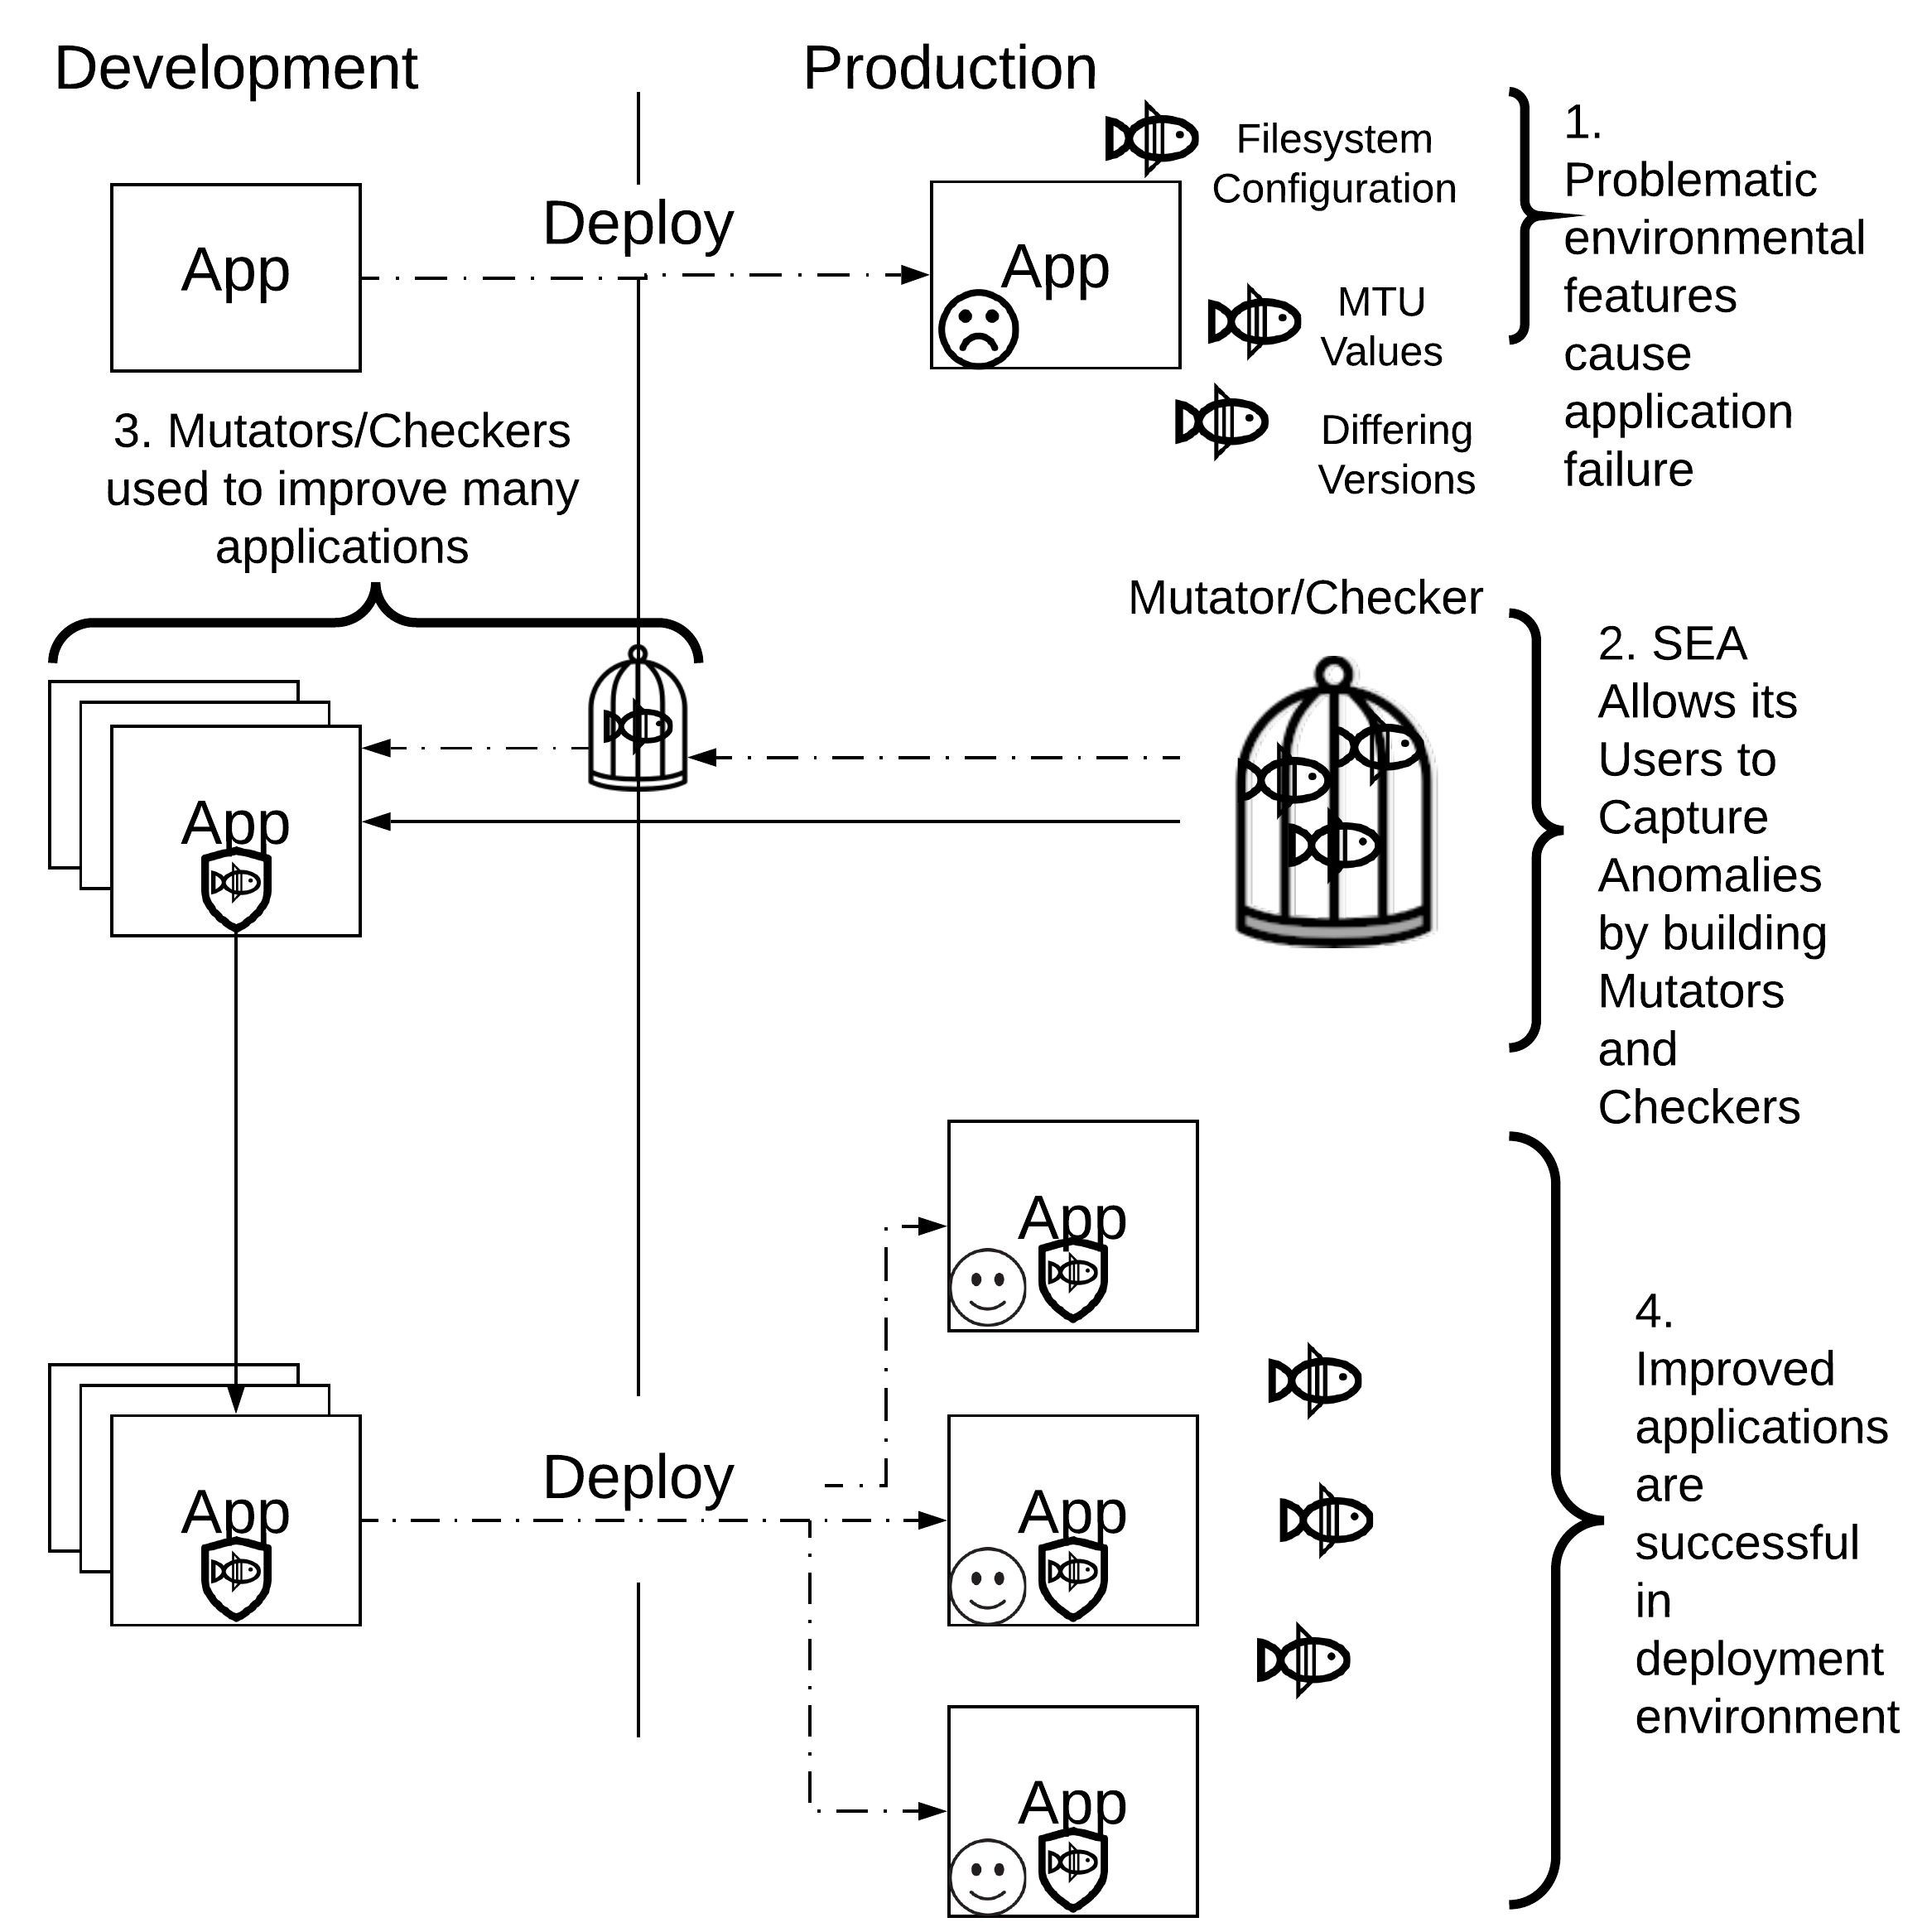
\includegraphics[scale=.6]{chapter3/images/approach}}
  \caption{Using SEA allows developers to capture features that make an
    environment problematic and use them to prevent future applications
    from falling victim to the bugs of the past.}
  \label{figure:approach}
\end{figure}

The Simulating Environmental Anomalies (SEA) technique
offers a methodical way to
capture, store, and utilize the insights gleaned from
previous failures in a given environment.
In this section, we offer a high-level look at how
SEA works, as illustrated in Figure~\ref{figure:approach}.
This is followed by a more in-depth look at its primary operations,
and the details of our concrete implementation, CrashSimulator.

\subsection{SEA in a Half-shell}
\label{SEC:SEAHalfshell}
In brief,
here is how the technique works.
An application, $A$, is run
in a particular environment and fails.
In debugging the failure,
we identify and ``trap'' the particular environmental feature
(sec.~\ref{SUBSUB:IdentifyingAndEncoding}),
that caused the failure,  which we call $X$.
We verify that when $X$ is present,
the results of interactions with the
environment are different,
sometimes in a barely perceptible manner,
and other times in a radically contrary manner.
We call this difference $\Delta X$.
$\Delta X$ can be extracted, preserved,
and later used in testing other applications
thanks to a pair of components referred to as a mutator and a checker.
The mutator, $mutX()$,
is able to apply $\Delta X$
to the appropriate places in an application's interactions
in order to simulate the presence of $X$.
The checker, $checkX()$ describes how an
application should respond once $X$ has been encountered.
To test if another application, $B$, also has a problem with $X$,
$mutX(B)$ is used to apply $\Delta X$ to its interactions
(sec.~\ref{SUBSUB:MutatingCommunications}).
$checkX(B)$ is then used to determine whether
$B$ has responded correctly to $X$(sec.~\ref{SUBSUB:CheckingResponse}).
If the checker accepts $B$'s behavior
after $X$ is simulated,
we report it has been handled correctly.
If the checker doesn't accept, we report that it has not responded correctly.
Once created,
these pieces act as the persistent medium in which the details of
a given anomaly are stored.

Representing an anomaly in terms of mutators and checkers
allows it to be easily reused to test other applications
without per application effort.
While an application's test suite is typically
tightly coupled to the programming language
and frameworks with which it was written,
SEA's approach is agnostic to these features.
This means anomalies that were useful in testing one application
can be programmatically applied toward testing another.
In this way, SEA is able to augment application-specific test suites
by both decreasing the number of tests
that must be manually constructed
to cover environmental concerns
and by offering the possibility of catching
failures that had not been considered.
These anomalies can be accumulated from many applications
resulting in the ability to test new applications
against an ever increasing
set of problematic conditions.

\subsection{Primary Operations}
\label{SEC:PrimaryOperations}

To take a closer look at how SEA functions,
we divide the technique
into its three primary operations.
These are:
identifying and trapping anomalies,
mutating system call results,
and checking application responses.

\subsubsection{Identifying and Encoding Anomalies}
\label{SUBSUB:IdentifyingAndEncoding}
Building a corpus of anomalies
is an ongoing process that improves the technique's
effectiveness by extending the set of problematic features it can simulate.
Anomalies can be sourced
in a number of ways,
such as
examining the failures of other applications
in a target deployment environment,
or by using other tools that can identify
potentially problematic behavior in other domains~\cite{Zhuang_NSDI_2014,
rasley2015detecting}.
Another option is taking this information from
public bug trackers, which is ideal
if you wish to determine
whether or not an application
is vulnerable to a widely publicized bug.

The chosen anomalies are examined
to determine how they change the results
of system calls an application makes as
compared to a normal execution.
Once teased out,
these differences delineate
a set of modifications
that must be made to an execution
in order to simulate the chosen anomaly or anomalies.
These details are used to
construct both a mutator and a checker.
The mutator encodes
a description of when in execution an anomaly can be simulated,
as well as details of how to conduct that simulation.
The checker
(or set of checkers)
stores a characterization of
how the application should respond.
Describing anomalies in this fashion
allows them to be recorded systematically and cataloged for future use.

As an example, consider
an anomalous environment
where access to a required file is denied because of
the environment's file security configuration.
With this anomaly,
attempts to access the file,
such as
the {\tt read()} system call,
will fail with an error stating that access to the file is denied.
The mutator derived from this issue would be constructed to
identify similar accesses as opportunities
to insert the anomaly
by making these
accesses return ``access denied''.
As described in \ref{SUBSUB:CheckingResponse},
an associated checker would be built to
examine the application's behavior after a simulation and assess its
correctness.
Preserving the details of anomalies like this in the form of
mutators and checkers
allow them to be
easily used
to test responses of future applications.

Constructing new checkers and mutators is a creative process not unlike
writing a unit test.  The writer must understand both the cause of
misbehavior in a deployment environment and how it is visible in the
results of the system calls an application makes.  Once they have this
understanding, the actual construction boils down to building state
machines that recognize the required patterns of system calls.  As a
result, effort required by this process depends on the complexity of the
anomaly being simulated and the proficiency of the writer with the above
concepts.

\subsubsection{Mutating System Call Results}
\label{SUBSUB:MutatingCommunications}
Simulating an environmental anomaly requires specific interventions at the
correct moments during an execution.
These situations are identified
with the help of the chosen anomaly's
mutator.
For our work,
this means providing
the mutator
with the system calls
an application makes
so it can identify sequences
indicative of such opportunities.
At the appropriate time,
the application's system calls
are intercepted
and the mutator's anomaly description is used to
make the modifications necessary
to simulate the anomaly.
In the simplest case,
simulating an anomaly only requires
the modification of a single value
(e.g. {\tt read()} returning -1 rather than the number of bytes read).
We even found use for a ``null mutator''
that performs no mutation, but gives other tools an opportunity to examine an execution.
In more complex cases,
large numbers of diverse system calls
will need to be interdicted and altered
in order to provide a correct simulation.
The above file access scenario, for example,
requires the modification of a single system call.
Simulating something more complex,
like an unreliable system clock,
requires that all efforts
to access the clock
be modified to reflect the chosen aberration.

\subsubsection{Checking an Application's Response}
\label{SUBSUB:CheckingResponse}
SEA relies on checkers
to provide a flexible approach to assess the way an application
behaves after it has encountered an anomaly.
A checker models
the behavior an application should undertake
in response to a simulated anomaly.
It looks for this behavior by examining an application's system calls
before, during, and after simulation.
The checker then reports whether the application has handled
the anomaly correctly
based on whether it observed the behavior for which it was built to look.

As an example, consider the ``default checker'' from CrashSimulator.
It draws a conclusion based on
whether or not the application
has made an effort to respond
to the anomaly.
This determination is made based
on the assumption
that such a response will yield
different program paths, and therefore different system calls.
If the application
does not alter its behavior, it has not
correctly handled the anomaly.
Alternatively,
if the application does deviate,
it is likely
an action has occurred to handle the simulated condition.
This simple yes or no approach
is often sufficient
to classify application behavior.

We explore this, and other checkers in our
Evaluation section (Section VI)~\ref{sec:SEAevaluation}.
Section~\ref{sec-move-bugs} demonstrates how to find bugs using the null
mutator, while Section~\ref{sec-file-type-bugs}
illustrates how a more complex
mutator can simulate specific scenarios to see if unexpected problems
emerge.


\subsection{CrashSimulator: A Concrete SEA Implementation}
\label{SUBSEC:ApproachCrashSim}

In order to correctly implement SEA, CrashSimulator
must provide a framework
by which the checkers and mutators
constructed by its users can be used to
test an application using the anomalies they represent.
Building this capability
required making a few key design decisions. The first, as mentioned in
Section 2, was choosing to operate at the system call level, rather than
manipulating calls to library functions, memory accesses, or other points
where we could influence an application's interactions.
This allowed CrashSimulator
to test applications written in any
language that can execute Linux system
calls -- an important advantage as our
goal is a tool that can test many
applications without per application
effort.
Working with system calls is also a good fit
for simulating the file system,
network, and operating system anomalies in which we were interested.
An application normally queries these entities using system calls
so we simply had to return modified responses in order to simulate an
anomaly.
Finally, robust tooling in the Linux kernel made the
interception and modification of system call results and side effects a
fairly simple process,  and the well-defined semantics of Linux
system calls streamlined implementation.


In order to take advantage of our ability to simulate anomalies using
system calls, we needed to ensure that an application would reliably make
the same set of
system calls, and reach the same simulation opportunities,
with every execution.
To this end,
we employed a modified
{\tt rr} debugger~\cite{rrwebsite} to record and replay applications. Our
first modification permitted a {\tt strace}-style system call recording
to be output alongside {\tt rr's} normal recording format,
creating a complete log of an application’s system call activity.
We chose to make this
modification because, while {\tt rr}'s recording contains the system call
information we need, it is stored in an opaque format that changes
frequently between versions.  Storing a copy of this information as a {\tt
strace} recording bypasses this shortcoming and offers the advantage of
being human readable.

Our second modification parallelized our testing
by allowing {\tt rr} to generate copies of a running application when
it reaches our target simulation opportunities.
We refer to this new technique as {\it process set cloning}
and illustrate it
in Figure~\ref{figure:architecture}.
The {\tt rr}
debugger manages, and can copy, the full set of processes underlying an
application so that users can test debugging hypotheses without damaging
the original.  We extended this capability by liberating process
set copies from {\tt rr}.  This means that given application $Y$ consisting
of processes $a$, $b$, and $c$ (written as $Y(a, b, c)$), we can generate
cloned sets $Y_1(a_1, b_1, c_1)$, $Y_2(a_2, b_2, c_2)$ ... $Y_n(a_n, b_b,
c_n)$.  $Y_1$, $Y_2$ ... $Y_n$ can then be used to test different
scenarios.  These clones can be run in parallel because they do not
actually execute system calls or modify the operating system state.
Instead, they are simulated as described below.
Additionally,
they allow the original $Y$ to continue its execution unhindered.

Once generated, the cloned process sets are used
for testing by the CrashSimulator process supervisor.
This supervisor is responsible for attaching to a process set
via {\tt ptrace} and
servicing any system calls it makes.
The data required to service these calls
comes from the  {\tt strace} log
generated by {\tt rr}.
Just before it takes over service of system calls,
the process supervisor invokes the intended anomaly's mutator
on the log in order to alter it to include the responses
necessary to simulate an anomaly.
Once these alterations are in place,
the supervisor is able to impose an anomaly
on the application by returning the now-modified responses from the log.

During this process,
a corresponding checker
monitors the application's behavior,
allowing it to report on the correctness of the response.
For example, testing could proceed in the following way.
At a given simulation opportunity, when executing application $Y$,
cloned sets $Y_1$ and $Y_2$ are generated and
used to test two scenarios where a file access could fail:
\begin{enumerate}
    \item{For $Y_1$, access to the file is denied due to a permissions issue}
    \item{For $Y_2$, access fails because of an I/O error}
\end{enumerate}
The simulations for both $Y_1$ and $Y_2$ are handled asynchronously and
the results are recorded.
This approach allows many tests to be run independently of one another,
which lends a
high degree of speed and
parallelism to the testing process.
At the same time, the original $Y$ execution continues unhindered to the
next simulation opportunity where this process repeats.
Keeping the original execution intact,
as opposed to destroying it by introducing an error state,
avoids the penalty
of having to restart a new execution for each test.

\begin{figure}[t]
  \center{}
  \fbox{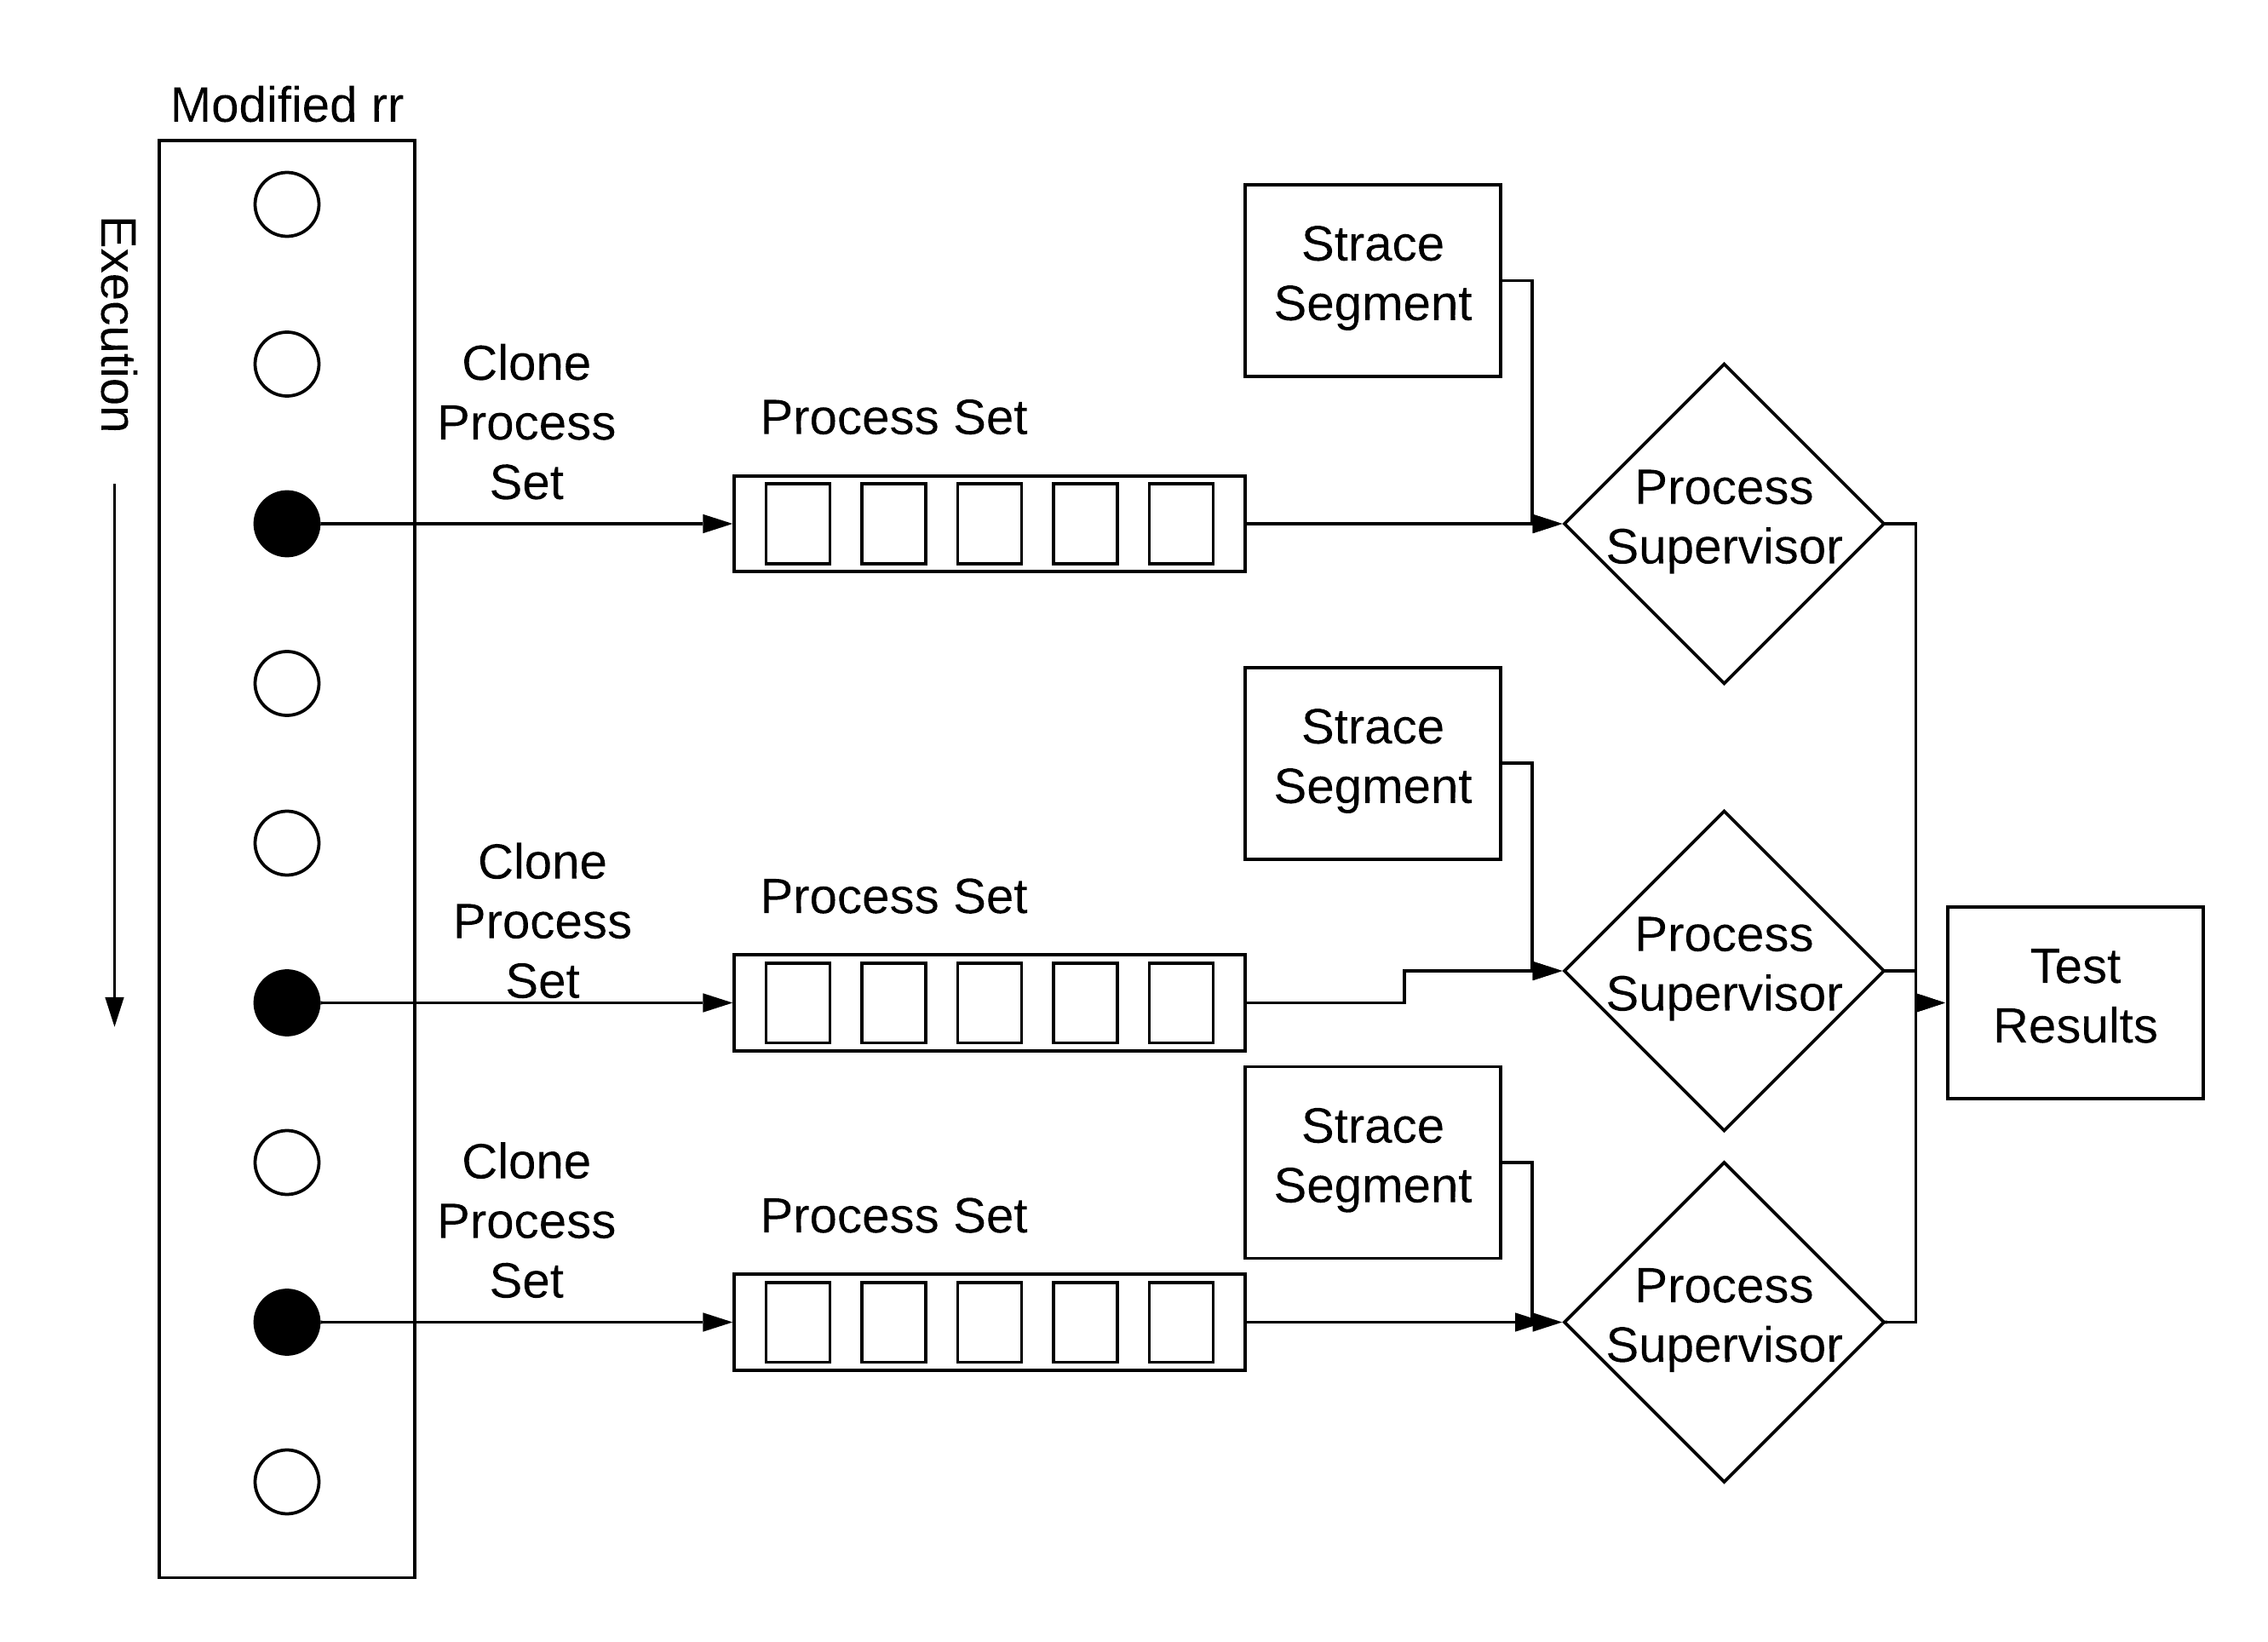
\includegraphics[scale=.70]{chapter3/images/architecture}}
  \caption{Diagram illustrating CrashSimulator's architecture.  During the
    course of a single rr execution, clone process sets are generated at
    specific rr events.  A CrashSimulator process supervisor attaches to
    these process sets and uses a strace-style system call listing to feed
    subsequent system call activity and inject unusual environmental
    conditions.}
  \label{figure:architecture}
\end{figure}

The prototype was built on rr version 5.2.0 running on a 32-bit Linux kernel
distributed with Ubuntu 16.04 LTS.  The modifications to rr described above
were carried out in C++, and the CrashSimulator
supervisor was implemented in 6260 lines of Python 2.7 code with a 2125
line C extension that allows it to interact with processes using the Ptrace
API.
This version of CrashSimulator is available at:
https://github.com/pkmoore/rrapper.

\input{chapter3/implementation}
\section{Evaluation}
\label{sec:SEAevaluation}

CrashSimulator was designed
as a way to reduce the considerable effort
required of developers to test an application
against the environments it will encounter once deployed.
Therefore,
we needed to demonstrate its effectiveness in ``the wild.''
To this end,
we carried out two rounds of
evaluation for CrashSimulator.
We started by exposing
a series of real-world applications
to a library of collected anomalies in a laboratory environment.
These tests,
conducted by the research team,
were followed by a user study
in which undergraduate and graduate computer science students
got a chance to use CrashSimulator
to identify new environmental bugs
in tests on applications of their choosing.
We used the results from both these efforts
to answer the following questions:

\begin{enumerate}

\item{Is CrashSimulator able to identify bugs in real world applications?
    (Subsection~\ref{sec-env-bugs})}

\item{What sorts of errors does CrashSimulator make?
    (Subsection~\ref{sec-sorts-errors})}

\item{Can CrashSimulator
      execute tests efficiently? (Subsection~\ref{sec-perf})}

\end{enumerate}

\subsection{Is CrashSimulator able to identify bugs in real world
applications?}
\label{sec-env-bugs}

The most crucial question to ask about the SEA technique and the tool we
implemented is:
can we use them to identify bugs
caused by different types of problematic environmental features?
To perform this evaluation we needed both a set of applications to test
and a set of anomalies against which to test them.
In order to show that CrashSimulator
can find bugs in even the most widely deployed
and well tested applications,
we chose our test candidates
from among those deemed ``popular''
by Debian's Popularity Contest~\cite{DebPopCon},
or those used
by many Linux distributions,
such as the ones provided
by the GNU coreutils project.

To prove the breadth of CrashSimulator's capabilities we needed
to test applications
using a diverse set of exemplar anomalies.
We already established
that
unusual filesystem and network situations can cause an application to fail.
So we identified a number of candidate anomalies
by examining public bug trackers,
the source code of major portable applications, and the capabilities of
bug finder tools like NetCheck~\cite{Zhuang_NSDI_2014}
and CheckAPI~\cite{rasley2015detecting}.
From these candidates we
chose to three test scenarios: a simple filesystem anomaly that relies on the null
mutator;
a more complex filesystem anomaly that simulates
the presence of unusual file types;
and a network anomaly that requires
checking and mutating many values across a variety of system calls.
Our experiences testing applications with these anomalies are detailed below.

\subsubsection{The simplest case - A Filesystem Bug Found With the Null Mutator}
\label{sec-move-bugs}
In our first test we decided to evaluate the tool in its simplest possible
configuration -- employing the {\bf ``null mutator.''}
This mutator takes no action and simulates no anomalous conditions.
It simply allows checkers to evaluate an application's behavior
as it carries out a potentially-buggy operation.
We decided to look at how applications
move files around on the filesystem.
Though, in many cases, this operation can be handled
atomically by the operating system
through the {\tt rename()} system call,
in situations where
the source file and destination file are on different storage devices,
the application must perform the operation in a more complex way.
This is a process
that even well-tested applications
frequently get wrong~\cite{PHPRenameBug,PythonShutilBug,NodejsCopyBug}.

{\bf Method.}
CrashSimulator was configured
to test each of the applications listed in Table~\ref{table:crossdevice}
to see which might fail to correctly move a file from one disk to another.
The tests were completed using just the Null Mutator and a set of
checkers that model the correct steps involved in moving a file from one
storage device to another.
After examining several libraries and applications,
we found that
{\tt mv} seemed to handle cases that other tools failed to consider.
Therefore, we
used its behavior as a template to create a set of checkers
that evaluate whether or not
the application correctly performs the following
steps.

\begin{itemize}
    \item{{\it Confirm Source Not Replaced During Copy.} An application
        should make an effort to ensure that the file being copied is not replaced between the time it is initially examined and when it is opened for copying.
If these checks are not performed, it
means the application will proceed with its operations,
        making file corruption~\cite{PythonShutilBug}} possible.

    \item{{\it Preserve Extended File Attributes.}
When copying a file,
an application should retrieve extended file attributes from the source
file and, later, apply them to the destination file.  Failure to do so can lead to security problems~\cite{AppleCodeSigning}.}

    \item{{\it Preserve Timestamps.}  It is important to ensure
that time related metadata --
such as creation, modification, and access times  --
are preserved when copying a file, as
incorrect timestamps can impede applications like {\tt make},
        archival programs, and similar software~\cite{NautilusTimestamps,
        SudoTimestamp}.}

    \item{{\it Copy Devices Correctly.}
Files of this variety must be moved
by creating a new device of the same type at the destination,
instead of exhaustively reading and writing its contents.
In our experience, applications that fail to perform this check
can end up completely filling disks, exhausting available memory,
        or blocking forever, which can cause the system to become unresponsive.}

\end{itemize}

 \begin{table}[t]
    \centering
    \begin{tabular}{l p{2cm} p{2cm} p{2cm} p{2cm}}
    \toprule{}
        Application     & Source Replaced & Preserve Xattrs & Preserve Timestamps & Copying Devices\\
\hline
        {\tt mv}              & Correct             & Correct             & Correct         & Correct\\
        {\tt mmv}             & Correct             & {\bf Sec. Flaw} & {\bf Time Loss} & Correct\\
        {\tt install}         & Correct             & {\bf Sec. Flaw} & {\bf Time Loss} & {\bf Fill Disk} \\
        {\tt perl File::Copy} & Correct             & {\bf Sec. Flaw} & {\bf Time Loss} & {\bf Fill Disk} \\
        {\tt shutils}         & {\bf Corrupt}       & {\bf Sec. Flaw} & Correct         & Correct\\
        {\tt rust}            & Correct             & {\bf Sec. Flaw}     & {\bf Time Loss} & {\bf Fill Disk} \\
        {\tt boost::copyfile} & {\bf Corrupt}       & {\bf Sec. Flaw}     & {\bf Time Loss} & {\bf Fill Disk} \\
    \bottomrule{}
    \end{tabular}
    \caption{Applications and libraries analyzed to determine whether or not
      they are able to correctly move a file from one device to another.
Incorrect entries are either missing the needed check to ensure correct
     behavior or their implementation of the behavior was ineffective.}
    \label{table:crossdevice}
\end{table}

{\bf Findings.}
CrashSimulator was able to identify whether an array of popular programs,
including the standard libraries for the programming languages Python,
Perl,
and Rust,
can correctly perform complex
operations in anomalous situations.
As can be seen from the results in Table~\ref{table:crossdevice}, each of the
applications tested failed to perform one or more of the steps required to
successfully complete a cross-device move.  This is an unfortunate situation
because a failure to perform any one of these steps can result in negative
outcomes for the system as a whole.  There was one case where our
checkers made a false positive report which prompted efforts to improve it.
This is discussed further in
Section~\ref{sec-sorts-errors}.
Taken as a whole, our results demonstrate that even well-tested applications
can miss one or more of the steps in a complicated operation.

\subsubsection{A More Complex Case - The Unexpected File Types Mutator}
\label{sec-file-type-bugs}

If a more complex mutator is to be employed, then
CrashSimulator will simulate anomalies as an application is executed.
This simulation introduces problematic scenarios
so an application's response
can be evaluated.
For an effective test of the
tool's capabilities to find bugs created in this process,
we needed to pick an anomaly
that would arise during a common situation,
such as when a Linux application retrieves
and processes data from a file.
Linux supports
several special file types,
including
directories,
symbolic links,
character devices,
block devices,
sockets, and
First-In-First-Out (FIFO) pipes.
These special files
use the same system calls
as regular files
(such as {\tt read()} and {\tt write()}),
but they behave in very different ways.
For example,
{\tt /dev/urandom} is a character device
that produces an infinite amount
of pseudo-random data
when read.
If {\tt /dev/urandom} is provided to an application
that relies on exhaustively reading the full
contents of a file before processing, it
will fill memory or disk space, and could
crash the system~\cite{YumAptEndless}.
Correct execution in these situations
requires that applications
examine the files, so they do not
interact inappropriately with a given file type.

{\bf Method.}
Identifying these bugs involves changing an application's
execution to induce its response to an unexpected file type. For
example, the {\tt sed} application, which modifies the contents of a text
file according to a provided command string, could instead be provided a symbolic
link, a directory, or a character device.  CrashSimulator
tests these alternatives by identifying the calls to {\tt stat()}, {\tt fstat()},
or {\tt lstat()} that an application makes to examine the file, and
changing the results to simulate
one of the special file types.  If the application responds to
this injected information, then the special
file might be handled correctly.  On the other hand, if there is no
alteration in the behavior of the application, the condition is not
being handled correctly.

For each application,
CrashSimulator was configured to simulate all of the non-standard file
types.
The values inserted into results of the application's {\tt stat()}-like
system calls are listed
in Table~\ref{table:unexpectedtypes}.
A value of ``--'' indicates
that this is the file type the application was expecting,
as it matches what was provided when the application was initially recorded.
A result of ``\tickmark'' indicates that the application
identified it was being provided with an unexpected file type and its
execution differs, a signal that it was potentially handling the
file type correctly.
A result of ``X'' indicates
that the execution never diverged from the trace being replayed,
and thus failed to recognize the presence of an unusual file type.

{\bf Findings.}
The data in Table~\ref{table:unexpectedtypes} show that of the 84 cases we
tested, CrashSimulator identified 46 bugs,
predicted 25 instances of correct application behavior,
and made 13 errors,
the majority of which were false negatives.
We discuss the causes of these errors
in Section~\ref{sec-sorts-errors}.
The frequency of failed executions in our results
indicates that many
applications assume they will only be used to process
regular files.  When this assumption does not hold, execution results
can be hard to predict.
In many cases a denial of
service condition occurs in the form of the application ``hanging,'' as it
attempts to incorrectly process the file.
This is typically the result of
an application blocking forever as it waits for a {\tt read()}
call to retrieve non-existent data from an empty FIFO,
or an application attempting
to read in and process an
``infinitely large'' file.
This situation is particularly dangerous as
it can eventually
fill all available memory or disk space~\cite{Cappos_CCS_08}.


\begin{table*}[t]
    \scriptsize{}
    \centering
    \begin{tabular}{l  l  |  p{1cm}  p{1cm}  p{1cm}  p{1cm}  p{1cm}  p{1cm} p{1cm}}
    \toprule{}
        Application       & Condition Tested           & Regular File           & Directory               & Character Device        & Block Device           & Named Pipe                 & Symbolic Link             & Socket File \\
                          &                            &  (IFREG)               & (IFDIR)                 & (IFCHR)                 & (IFBLK)                & (IFIFO)                    & (IFLNK)                   & (IFSOCK)\\
\hline
        {\tt Aspell}      & Dictionary File            & --                     & X: \textit{FP}          & \tickmark: \textit{FN}  & X                      & X                          & X                         & X          \\
        {\tt Aspell}      & File being checked         & --                     & X: \textit{FP}          & \tickmark               & X                      & X                          & X                         & X          \\
        {\tt gnu-gpg}     & secring.gpg                & --                     & X                       & X                       & X                      & X                          & X                         & X          \\
        {\tt vim}         & File being opened          & --                     & \tickmark: \textit{FN}  & \tickmark: \textit{FN}  & \tickmark: \textit{FN} & \tickmark: \textit{FN}     & \tickmark: \textit{FN}    & X          \\
        {\tt nano}        & File being opened          & --                     & \tickmark               & \tickmark               & \tickmark              & X: \textit{FP}             & X: \textit{FP}            & X: \textit{FP} \\
        {\tt sed}         & File being edited          & --                     & \tickmark               & X: \textit{FP}          & X                      & X                          & X                         & X          \\
        {\tt wc}          & File being checked         & --                     & \tickmark               & X                       & X                      & X                          & X                         & X          \\
        {\tt du}          & Directory being checked    & \tickmark              & --                      & \tickmark               & \tickmark              & \tickmark                  & \tickmark                 & \tickmark  \\
        {\tt install}     & File being installed       & --                     & \tickmark               & X                       & X                      & X                          & \tickmark                 & X          \\
        {\tt fmt}         & File being formatted       & --                     & X                       & \tickmark               & X                      & X                          & X                         & X          \\
        {\tt od}          & File being dumped          & --                     & \tickmark               & \tickmark               & X                      & X                          & X                         & X          \\
        {\tt ptx}         & File being read            & --                     & \tickmark               & \tickmark               & \tickmark              & \tickmark                  & \tickmark                 & \tickmark: \textit{FN} \\
        {\tt comm}        & Second file being compared & --                     & \tickmark               & \tickmark               & X                      & X                          & X                         & X          \\
        {\tt pr}          & File being read            & --                     & \tickmark               & X                       & X                      & X                          & X                         & X          \\
\hline
        \multicolumn{9}{l}{\scriptsize{\tickmark  $=$ CrashSimulator
        predicts application will recognize anomaly}}\\
        \multicolumn{9}{l}{\scriptsize{X $=$ CrashSimulator predicts
        application will fail to recognize anomaly}}\\
        \multicolumn{9}{l}{\scriptsize{-- $=$ File type expected by the
        application}}\\
    \bottomrule{}
    \end{tabular}
    \caption{Applications tested for their handling of unexpected file types.  A
    result of ``\tickmark'' indicates that the application identified the
    presence of an unusual file and responded in some fashion.  A result of
    ``X'' indicates that the application failed to recognize the presence of
    an unusual file and attempted to process it.  Cases where
    CrashSimulator made an error are noted by FP (False
    Positive) or FN (False Negative)}
    \label{table:unexpectedtypes}
\end{table*}


\begin{table}[t]
    \centering
    \begin{tabular}{l  l  l  l  l  l  l  l  l}
    \toprule{}
        Application         & Directory                 & Character Device & Block Device  & Named Pipe \\
                            & (IFDIR)                   & (IFCHR) & (IFBLK) & (FIFO) \\
\hline
        {\tt wc}            & Error: Is a Directory     & hangs       & slowly process file  & Hangs\\
        {\tt install}       & Error: Omitting Directory & Fills disk  & slowly copies file   & Hangs\\
        {\tt fmt}           & No output                 & hangs       & garbage output       & Hangs\\
        {\tt od}            & Error: read error         & hangs       & No output            & Hangs\\
        {\tt ptx}           & Error: Is a Directory     & fills disk  & garbage output       & Hangs\\
        {\tt comm}          & Error: Is a Directory     & hangs       & garbage output       & Hangs\\
        {\tt pr}            & Error: Is a Directory     & hangs       & garbage output       & Hangs\\
\hline
    \bottomrule{}
    \end{tabular}
    \caption{Responses of a sample of coreutils applications when exposed to
      anomalous conditions.  The character device used was the infinite-length {\tt
        /dev/urandom}.}
    \label{table:applicationresponses}
\end{table}

In order to confirm the accuracy of CrashSimulator's assessment, we manually
exposed the applications listed in Table~\ref{table:unexpectedtypes} to
each of the unusual file types to get an idea of how they would respond.
This allowed us to identify cases where CrashSimulator made errors and
note this information in Table~\ref{table:unexpectedtypes}.  Further,
we include descriptions of a subset of the applications' behaviors in
Table~\ref{table:applicationresponses}.
These tables serve to document the accuracy of the tool's
evaluation of application behavior and illustrate what misbehavior occurs
when applications are actually exposed to problematic scenarios.
%One possibility is that CrashSimulator asserts
%that the application will fail
%and in practice, it does.  We found this when we evaluated
%the response of  {\tt install} receiving a character device
%rather than a regular file. Our test predicted failure and the
%application ended up filling the disk of the machine on which it was run.
%In other cases, CrashSimulator reported that an
%application had detected the anomalous condition and the application managed to
%do so in practice,  as when we evaluated {\tt wc}'s successful response to
%being run on a directory.

\newgeometry{left=3cm}
\begin{figure}[btp]
\centering
\begin{lstlisting}
  @@ -1006,16 +1006,20 @@ void check()
      exit(1);
    }
  
  - #ifdef USE_FILE_INO
     {
      struct stat st;
  +   fstat(fileno(in), &st);
  +   if (!S_ISREG(st.st_mode)) {
  +     print_error(_("\"%s\" is not a regular file"), file_name);
  +     exit(-1);
  +   }
  + #ifdef USE_FILE_INO
      int fd = open(new_name.c_str(),
                    O_WRONLY | O_CREAT | O_TRUNC, st.st_mode);
      if (fd >= 0) out = fdopen(fd, "w");
  - }
    #else
  - out = fopen(new_name.c_str(), "w");
  + out = fopen(new_name.c_str(), "w");
    #endif
  + }
    if (!out) {
      print_error(_("Could not open the file \"%s\" for writing.
      File not saved."), file_name);
      exit(-1);
\end{lstlisting}
\caption[Aspell Patch]{This listing shows a patch that corrects a deficiency in Aspell.  Lines 8 through 12 add a new check that ensures Aspell will stop execution rather than attempt to process any non-regular file
(i.e. a file for which fstat() returns a
ST\_MODE value that is not S\_IFREG).
Prior to this patch's acceptance, Aspell would hang and fill the local disk with garbage data when processing an unusual file such as /dev/urandom}
\end{figure}
\restoregeometry

\subsubsection{Beyond Filesystem Bugs - Poorly Configured Network Timeouts}
\label{sec-timeout-bugs}

CrashSimulator is not limited
to identifying filesystem-based bugs.
The third anomaly we examined
involves an application's behavior
when it attempts to communicate
over a network with extremely long
(on the order of minutes) response times.
At a low level,
applications retrieve data from a network socket
by waiting for data to be available and then reading it.
However,
this approach needs to be able to handle
a situation where communication
takes too long and should time out.

{\bf Method.}
CrashSimulator can detect
whether an application correctly times out when communications
take too long
by employing the null mutator and a network timeout checker. The latter
can determine if the application makes any effort
to configure its network communications with a timeout value.
This is done by examining the presence or absence of {\tt setsockopt()}, {\tt poll()}
and {\tt select()} calls, as well as the timeout values that may
have been passed to them. Applications that do not set the timeout are
subject to the operating system-defined protocol timeout value.
CrashSimulator is able to take this analysis a step further by employing a Long Network Response Time mutator
that manipulates
the results of all time-returning calls,
simulating an execution where close to the maximum timeout value occurs,
without actually spending any time waiting.

An application's failure
to time out responsibly
is not just an inconvenience. Attackers can take advantage of this flaw
to consume resources and potentially cause a denial of service situation.
This failure was exploited by the slowloris~\cite{Slowloris} tool
to enhance the ability
of a small number of computers to prevent access
to vulnerable web servers
by opening and maintaining connections
for extremely long periods of time.
As these servers could only handle a set number of connections
due to resource constraints,
legitimate traffic was easily crowded out by the attackers.
Additionally, similar attacks can be used to
indefinitely delay security updates to
clients, leaving them vulnerable to compromise~\cite{Cappos_TR_08}.
We used CrashSimulator to determine which applications and
libraries from a selection based on Debian's ratings~\cite{DebPopCon}
could be vulnerable to this sort of attack.

\begin{table}[t]
    \centering
  \begin{tabular}{l | l}
    \toprule{}
    {\bf Application}              & {\bf Analysis Result}\\
    {\tt wget}                     & Overly long timeout supplied to {\tt select()} \\
    {\tt ftp}                      & No {\tt poll()} or {\tt select()}, no timeout set \\
    {\tt telnet}                   & {\tt select()} specifies no timeout \\
    {\tt urllib http}              & No {\tt poll()} or {\tt select()}, no timeout set \\
    {\tt urllib ftp}               & No {\tt poll()} or {\tt select()}, no timeout set \\
    {\tt ftplib}                   & No {\tt poll()} or {\tt select()}, no timeout set \\
    {\tt httplib}                  & No {\tt poll()} or {\tt select()}, no timeout set \\
    {\tt requests}                 & No {\tt poll()} or {\tt select()}, no timeout set \\
    {\tt urllib3}                  & No {\tt poll()} or {\tt select()}, no timeout set \\
    {\tt python-websocket-client}  & No {\tt poll()} or {\tt select()}, no timeout set \\
    \bottomrule{}
  \end{tabular}
  \caption{Applications tested for their handling of extremely slow response
    times from the host with which they are communicating }
  \label{table:slowloris}
\end{table}


{\bf Findings.}
As Table~\ref{table:slowloris} shows, all of these
applications were vulnerable to this anomaly,
and in some cases,
timeouts took hours to resolve.
What's more, in the vast majority of
cases, the problem occurs because the application makes no effort to
specify a timeout value.  This means an attacker can transmit one byte of
data per timeout period (per Linux's value of 19 minutes for TCP sockets),
allowing them to keep the application alive instead of quitting.

\subsubsection{Bugs Found By Participants}
Because the above tests were carried out by CrashSimulator's developers,
who necessarily have a high degree of expertise in its operation,
we felt it prudent to ensure the tool was useful
to outside developers as well.
To investigate this angle,
we conducted a user study
with 12 undergraduate and graduate students with varying backgrounds.
Study participants found a total of 11 bugs using CrashSimulator.
Of these bugs, nine were found using the ``Unusual Filetype'' mutator.
Five of these bugs have since been reported to the appropriate maintainers,
and three of these reports included patches
that correct the bug
built by the reporting student.

These results are important
because they confirm
users, other than the original development team,
can use the tool to find bugs in real world applications.
Participants commented that narrowing the source of a bug
down to a particular sequence of system calls
was helpful in identifying the area of
code responsible for the bug -- a feature
that decreased the time required to produce a fix.
Though observation of study participants
showed that familiarity with operating systems concepts
made it easier to work with CrashSimulator,
those without this background were still able to identify bugs using the
built in anomalies.

On a less positive note,
the study did reveal
some shortcomings
of the tool.
First,
it became clear that the tool
does not have a clear mechanism
for determining
which application behaviors constitute a ``bug.''
For example, an application's developer
may have intended that an application processing an ``infinitely long'' file should run continuously
until killed by an outside command.
Therefore, that behavior should not be classified as a bug.
Second,
it demonstrated that
simply reporting that an application did or did not change its behavior
in the presence of an anomaly may not provide sufficient data to identify a bug. The results indicating the presence of a bug must be clear to the user.
Both of these issues are being corrected
by improving the tool's outputs.
By more clearly describing
the nature of a given result,
users can have a better idea
if,
and why,
they should be concerned.


\subsection{What Sorts of Errors does CrashSimulator Make?}
\label{sec-sorts-errors}

Like other testing tools, CrashSimulator occasionally makes mistakes.
Any such mistakes can
undermine a developer's confidence in a tool, and thus one of our goals is
to minimize them.   In this section, we discuss
situations where CrashSimulator made either false positive or false
negative reports.  A false positive report means the tool reports
a failure when the application actually handles an anomaly correctly.
On the opposite side, false negative reports happen when the tool indicates an application handles
an anomaly when, in reality, it does not.

\paragraph{False Positives.}
The primary source of false positives in CrashSimulator is an application
responding to an anomaly with a different sequence of system calls
than was expected by the checker.
Once identified, CrashSimulator's approach allows these
situations to be easily corrected.
This is similar to a situation
where an application's test suite
has a test with an over-constrained ``oracle''
(e.g. an oracle that ensures a returned value is $>0$ when, in reality,
$0$ is acceptable).

We encountered this situation when testing applications that used
GNOME's {\tt glib} file handling functions.  When an
application makes use of these facilities to move a file across storage
devices, the library itself correctly performs a
file move operation.  When we used CrashSimulator with
checkers that expected a call to {\tt read()} and {\tt write()}
for a cross-device move, we got reports stating that the
application {\em did not} perform the system calls necessary to
correctly move a file.
By manually
examining a system call trace, we found that, while {\tt glib} correctly
performs the requested move operation,
it does so using alternative system call
sequences.  Rather than using a sequence of {\tt read()} and {\tt write()}
calls, as our checker expected, {\tt glib} creates a pipe and uses the {\tt
splice()} system call to copy the contents out of the source file, through
the pipe, and into the destination file.

Fortunately, as soon as issues like this are discovered,
CrashSimulator's checkers can be modified to include the alternative
sequence.
Given the above example about moving
files, consider the mapping from high level ``operation'' to the set of
system calls that can implement it in Table~\ref{table:stepsandcalls}.
Each of the steps in the operation map to a small number of system calls.
In
situations where two system call sequences can correctly implement the same
operation, CrashSimulator simply runs two checkers in parallel
and accepts the execution if either detects the expected sequence.

\begin{table}[t]
    \centering
    \begin{tabular}{l | l }
    \toprule{}
      {\bf Operation}                                               & {\bf Potential System calls}\\
      Examine source file                                           & stat64(), lstat64(), fstat64()\\
      Examine destination file                                      & stat64(), lstat64(), fstat64()\\
      Open source file                                              & open()\\
      Read contents of source file                                  & read(), splice() with a pipe\\
      List source file's extended file attributes                   & listxattr(), llistxattr(), flistxattr()\\
      Read contents of source file's extended file attributes       & getxattr(), lgetxattr(), fgetxattr()\\
      Open destination file                                         & open(), optionally unlink() the file first\\
      Write contents to destination file                            & write(), splice() with a pipe\\
      Apply extended file attributes to destination file            & setxattr(), lsetxattr(), fsetxattr()\\
      Apply proper timestamps to destination file                   & utimens(), futimens()\\
      Apply proper permissions to destination file                  & chmod(), open() with a modeline specified\\
      Close the source file                                         & close()\\
      Close the destination file                                    & close()\\
    \bottomrule{}
    \end{tabular}
    \caption{Each step of a successful cross-disk file move operation mapped to
      the system call or calls that can implement it}
    \label{table:stepsandcalls}
\end{table}

%A second source of false positives is a test being configured such that not
%enough of the application's execution is included in the test.
%One implementation detail of CrashSimulator is that,
%by default,
%its tests evaluate an application's behavior
%within a defined (but configurable) number of system calls.
%We found in some cases
%that an application's error handling or recovery code
%may take place outside of this span of execution.
%False positives
%of this sort
%are easily corrected
%by expanding the length of execution
%covered by the test.
%The low number of occurrences of this
%type of false positive gives us confidence that the default configuration
%is satisfactory in the majority of cases.

\paragraph{False Negatives.}
False negatives are a fact of life in testing
because of missing test cases or under-constrained checks
of result correctness.
CrashSimulator occasionally registers  false negative reports
when an application changes its behavior,
but does not handle an anomaly correctly.
In our evaluation we encountered ten such reports, four
occurring with one application, {\tt wc}.
Because these reports were generated when using the default checker,
they can be addressed by
using a more elaborate checker that
performs a detailed analysis
of the application's post-simulation behavior.
Such a checker would compare this behavior to a model of
a correct response to that anomaly.
Creating this checker requires
that a user know
what a ``correct response''
looks like.
This ``known good'' behavior can be found
by looking at standards and documentation
that describe best practices for handling an anomaly
in a given environment,
or by examining how applications that correctly
deal with the anomaly do so.
Consider the case where a {\tt close()} system call fails.
Retrying the call may not be the correct action,
depending upon the environment in question.
SEA can be used to determine if an application
has handled the failure correctly
by examining post-simulation communications in detail,
and taking into account the correctness of retrying the call.

\subsection{Can CrashSimulator execute tests efficiently?}
\label{sec-perf}

One key attribute of successful testing tools is that they are able to
complete their tests in a timely manner.  If a tool takes too long,
users will be less likely to run it.
To address this concern,
we evaluated CrashSimulator's performance
in order to determine whether or not it was able to complete its
test executions in an acceptable time frame.

{\bf Method.}
To answer the question of performance, we examined the completion
times for executions of the specified application in both
native conditions, and under CrashSimulator configured to test using the ``Unusual File
Types'' anomaly discussed earlier.
Table~\ref{table:performance} shows these results.

 \begin{table}[t]
     \centering
     \begin{tabular}{l p{2cm} p{2cm} p{2cm} p{2cm}}
    \toprule{}
        Application     & Native Execution Time & Initial Recording Time & CrashSim. Replay Time & rr Replay Time  \\
\hline
        {\tt wc}        & 0m0.007s              & 0m0.473s               & 0m0.668s                   & 0m0.112s        \\
        {\tt fmt}       & 0m0.007s              & 0m0.321s               & 0m0.707s                   & 0m0.111s        \\
        {\tt od}        & 0m0.036s              & 0m0.317s               & 0m0.689s                   & 0m0.101s        \\
        {\tt ptx}       & 0m0.008s              & 0m0.352s               & 0m0.769s                   & 0m0.087s        \\
        {\tt comm}      & 0m0.132s              & 0m0.371s               & 0m0.776s                   & 0m0.141s        \\
        {\tt pr}        & 0m0.135s              & 0m0.888s               & 0m1.017s                   & 0m0.141s        \\
    \bottomrule{}
    \end{tabular}
    \caption{This table contains the times required to execute several coreutils applications under different conditions.
             Native execution time is the time required to execute the application from the command line while
             CrashSimulator Replay time is the time required to execute it with the tool, using the null mutator with no checker configured.
             Initial recording time is the time required to create an initial recording with CrashSimulator.  rr replay time is the
             time required to replay an application using rr without CrashSimulator and is included to demonstrate the additional
             overhead added by CrashSimulator's other components.}
    \label{table:performance}
\end{table}


{\bf Findings.}
Overall, the performance running an application
under CrashSimulator is around
two orders of magnitude slower
than the original program executed without it.
As can be seen in Table~\ref{table:performance}, around 20\%
of this slow down is related to the additional overhead of {\tt rr}'s replay.
An additional portion is caused by the need to spin up Python's interpreter
before testing can begin.
In most cases
this slowdown is somewhat mitigated by CrashSimulator's ability to process
tests asynchronously. In other situations, it will be more efficient than
running the program natively, as {\tt rr's} replay does not require
actual execution of most system calls.  This means that CrashSimulator
avoids the system call overheads, such as I/O.
Even without these improvements, however, CrashSimulator's performance
cost is more
than manageable when the value it provides is taken into account.  The
cumulative runtime required to execute the tests required to produce the
results listed in Table~\ref{table:unexpectedtypes} is around 90 seconds.

\section{Related Work}
\label{SEC:related-work}

In constructing SEA and CrashSimulator, we examined a number of previous
studies in bug detection, data mining, the influence of environment on
application behavior, and protocols for checking program responses to anomalous
situations. This section
summarizes a few earlier initiatives in each of these areas and discusses
their relevance to the development of our tool.

% One of the major limitations of many automated testing tools is a reliance
% on the availability of a target application's source code.  Out of the top
% XXX automated testing tools (as ranked by YYYY), ZZZZ have this
% dependency.\preston{cite} While open source software has dramatically
% increased in popularity over recent years, closed source dependencies are
% still a major concern.\preston{cite}  Any tool that requires access to
% source code will have diminished capability in projects incorporating
% closed source components.


\iffalse
While there is a vast amount of literature on test
generation~\cite{ammann2008introduction, mcminn2004search,
  puasuareanu2009survey, dias2007survey}, much less work
has focused on issues of portability, and tests of whether software
behaves consistently in different environments.  Prior work on
CheckAPI~\cite{rasley2015detecting} and
NetCheck~\cite{Zhuang_NSDI_2014} begins to fill this gap and this paper
builds upon those results.
%
%\paragraph{Detecting Environmental Bugs.}
%
%NetCheck; CheckAPI; stub injection; detecting machine specific bugs
%(e.g. numeric/memory limitations); testing error handlers; \dots


Crash reproduction by test case mutation~\cite{DBLP:conf/sigsoft/XuanXM15}.

\fi


\noindent
{\bf Static analysis. }
\label{rel-static-analysis}
Tools based on static analysis techniques, such as abstract interpretation,
model checking, and symbolic execution, have been successfully
used to
detect bugs resulting from incorrect API usage. Examples of these tools
include
SLAM~\cite{Ball_adecade, Ball:2002:SLP:503272.503274} and, more recently,
CORRAL~\cite{DBLP:conf/sigsoft/LalQ14} for conformance checking of Windows
device drivers against the Windows kernel API,
FindBugs~\cite{DBLP:conf/oopsla/HovemeyerP04} for detecting API usage bugs
in Java programs, FiSC~\cite{Musuvathi04modelchecking} for finding bugs in
TCP implementations, and the Explode
system~\cite{Yang:2006:ELG:1298455.1298469} for detecting crash recovery
bugs in file system implementations.  Likewise, INFER has found success at
Facebook in analyzing units of code as they are
committed~\cite{INFERFacebook}. Unlike CrashSimulator, these
approaches depend on the availability of source or byte code.

Static analysis techniques have also been
used to detect portability issues related to what happens when an
application encounters different
versions of the external components on which
it depends~\cite{silakov2010improving, javacompliance-www}. Like
CrashSimulator, these techniques
address the application's interactions with its
environment. However, these studies were focused on proving that the
environments behaved as expected.
CrashSimulator is only interested in the application's
response to anomalies.

\iffalse
\noindent
{\bf Specification and run-time verification.}
Substantial work has been done in validating API and protocol behaviors,
e.g., finding faults in the Linux TCP implementation, SSH2 and
RCP~\cite{Udrea:2008}, BGP configuration~\cite{Feamster:2005}, and
identifying network vulnerabilities~\cite{ritchey-sp00}.
\fi

\noindent
{\bf API protocol mining.}
Extensive work has been done on mining source code to learn API protocols
and use them to detect common usage violations, such as missing method calls
(see, e.g.,~\cite{mariani2007compatibility,
DBLP:journals/ase/WasylkowskiZ11, DBLP:conf/icse/PradelJAG12,
DBLP:journals/tosem/MonperrusM13, DBLP:conf/icse/JamrozikSZ16}). These
techniques primarily target object component interactions, rather than
system calls to generate test suites. However, the techniques explored in
these works could be used to mine system call patterns in source code.
This will enable researchers
to find checkers that identify incorrect responses to environmental
anomalies. So far, we have specified these checkers manually for
CrashSimulator.  Data mining techniques could be adapted in the years
ahead to reduce the manual effort required.

\noindent
{\bf Tracing and log mining.}
Similar to API protocol mining, substantive work has been done using
log files to detect anomalies~\cite{pinpoint,
jiang_abnormal_trace_detection_icac_2005, xu2009detecting, lou2010mining2}
and to aid in program understanding~\cite{yuan2010sherlog,
beschastnikh_synoptic_fse_2011, csight_icse_2014}.
For example, CheckAPI~\cite{rasley2015detecting}
and NetCheck~\cite{Zhuang_NSDI_2014} both
use system call traces to diagnose an application's violations of
cross-platform portability.  CrashSimulator in some ways takes these
techniques a step further by using
system call traces
to test responses to known environmental anomalies.
This more active approach can expose bugs that
are invisible to passive log mining.


\noindent
{\bf Environmental influence and cross-platform portability.}
Negotiating the influence of the environment in which an
application is deployed has been investigated from several
perspectives. One approach, referred to previously,
is to build ``portable'' systems
that have cross-platform capabilities.
Using wrapper subroutines
can enable cross-platform portability
of APIs~\cite{bartolomeicompliance} through system call delegation.
These wrappers can be automatically generated through techniques like
system call interposition~\cite{Guo:2011:CUS:2002181.2002202}, a
technique that can also be used to detect and prevent security
violations~\cite{Hofmeyr:1998:IDU:1298081.1298084,
Acharya:2000:MUP:1251306.1251307}.
Other works that target complementary classes of portability problems
include the detection of configuration-related bugs~\cite{skoll:icse:2004,
Yilmaz:issta:2004, Fouche:issta:2009, Kastner12, Nguyen14} and
cross-browser incompatibilities for web
applications~\cite{DBLP:conf/icsm/ChoudharyVO10, silakov2010improving,
DBLP:conf/icse/Choudhary11, Mesbah:2011:ACC:1985793.1985870,
DBLP:conf/icst/DallmeierP0MZ14}.  Static analysis tools, such as those
mentioned earlier in this section, have also been applied to
detection of differences between versions of external components.

Such studies have helped to define the influence of an environment on
applications and thus provide a background to our work.  Our tool applies
these fundamental ideas to testing an application's response to anomalies.

\noindent
{\bf Testing exception handling and conformance.}
A few researchers have developed testing techniques aimed at checking
whether programs respond appropriately to anomalous situations.  For
example, Fu et al. introduced data flow testing techniques that require
tests from the points at which exceptions are thrown to the points
at which they are handled in Java code. The purpose is to discover whether
programs respond correctly to exceptional situations anticipated by the
programmer~\cite{DBLP:journals/tse/FuMRW05}.  Koopman and DeVale developed
a system to detect bugs in error handling code related to calls to POSIX
functions~\cite{Koopman00theexception}.  Miller et al. cover the kernel as
a source of unexpected program inputs and test applications by simulating
them~\cite{murphyslaw}.
Other approaches to conformance checking of POSIX operations use model
based testing~\cite{Dadeau:2008:CSM:1433121.1433137,Farchi02}.

Unlike these approaches, CrashSimulator does not exclusively target error
handling code or anomalies that only involve individual system calls.
Additionally, it focuses on collecting and simulating
problematic features of specific
deployment environments.
That said, such testing techniques
can help identify additional anomalies  to add to our repository.

{\bf Smart Fuzzing.}
Smart fuzzers monitor and guide executions to
trigger code paths that are unlikely to be reached
otherwise~\cite{smartfuzzing, taintbasedfuzzing}.
At this point, they make a binary decision about
whether the application correctly handled the input or not.
Typically, a determining factor will be an actual crash by the application.
This is similar to SEA's use of checkers to decide whether
to accept or reject a given test
execution, based on whether or not it observed a specific system call behavior.
In both cases, the tools can demonstrate whether a given code path handles a
situation correctly, but cannot prove that the code path is robust against
other problematic inputs.  In the future, CrashSimulator could use smart
fuzzing path exploration techniques to generate tests that reach relevant
system calls and apply SEA at that point.

%\noindent
%{\bf Runtime verification:}
%Runtime verification (RV)
%techniques~\cite{DBLP:conf/rv/2010, Liu:2007:WCC:1973430.1973449, Lu_ASPLOS_2006,
%Archer:2007:ICT:1236360.1236382, Verbowski_OSDI_2006, Tucek_SOSP_2007,
%Park_ASPLOS_2009,DBLP:journals/jlp/LeuckerS09}
%can detect violations of properties on specific executions
%but do not show that the software satisfies the specification for every
%possible input or on every possible execution.
%Many of these techniques find general violations of
%properties, such as atomicity~\cite{Park_ASPLOS_2009, Verbowski_OSDI_2006}.
%Other RV techniques enable checking program-specific requirements
%usually specified with formal languages, such as automata or logic
%formalisms~\cite{DBLP:conf/vmcai/BarringerGHS04, DBLP:conf/kbse/GiannakopoulouH01}.
%
%Many RV approaches instrument code to capture relevant
%events or application state and insert executable
%assertions~\cite{Orso:2002:GSC:566172.566182, DBLP:conf/icse/ClauseO11,
%DBLP:books/sp/Liblit2007, Jin:2010:ISS:1932682.1869481, Barnett01spyingon,
%DBLP:journals/jss/BarnettS03}.
%However, inserting pre- and post-conditions obscures the fact that the
%specification can be treated as a parallel construct to the
%implementation~\cite{Barnett01spyingon, DBLP:journals/jss/BarnettS03}.
%Instead, an architecture can be used for runtime verification of .NET
%components by running the model and the implementation side-by-side,
%comparing results at method boundaries~\cite{Barnett01spyingon,
%DBLP:journals/jss/BarnettS03}.
%CheckAPI does not require application instrumentation, assuming a tracing
%mechanism exists in the API~\cite{strace, Cappos_CCS_10}.

%Like CheckAPI,
%several other (runtime and static) checking techniques
%allow the use of languages more familiar to
%programmers.
%The WiDS checker allows using a scripting language to specify properties of a
%distributed system~\cite{Liu:2007:WCC:1973430.1973449}.
%Contracts written in a C-like language can specify components for use
%in TinyOS applications~\cite{Archer:2007:ICT:1236360.1236382}.
%CheckAPI allows
%programmers to choose the language for PSI construction or simply to
%use an existing implementation. Lastly, work on deterministic
%replay~\cite{Viennot13} enables record-replay techniques on multi-core
%systems and could help improve CheckAPI-MT performance.


\iffalse
\noindent
{\bf Application-specific fault detection.}
Pip~\cite{reynolds2006pip} and Coctail~\cite{xue2012using} are distributed
frameworks that enable developers to construct application-specific models,
which have proven effective at finding detailed application flaws. However,
utilizing these methods requires a knowledge of what failure needs must
be acquired, and a specification of all relevant system properties. 
NetCheck diagnoses application failures without application-specific
models.  Khanna~\cite{khanna2007automated} identifies the source of
failures using a rule base of allowed state transition paths.
%However, it requires specialized human-generated rules for each
%application.
CrashSimulator leverages NetCheck's approach to simulate identified
anomalies in network behavior, file system behavior, and other environmental-specific conditions. This enables the tool to test
applications other than the ones with which the anomalies were originally
discovered.
\fi


%% The following is old stuff -- not sure how much should be integrated
%% into the above.
\begin{comment}
\subsection{Existing Techniques}

Existing tools can be roughly divided into two categories, black-box
and white-box, based on the techniques they use to perform their
testing. Black-box tools simply manipulate the inputs of the
application under test and observe the resultant outputs. White-box
tools, on the other hand, perform complex analysis of the application's
source code in order to reason about what inputs are likely to produce
interesting outputs. Each of these methodologies have their own
advantages and disadvantages.

White-box testing tools typically rely on a similar set of techniques,
including constraint solving of branch statements in an application's
code and symbolic execution of an application's code in order to
generate inputs that optimally exercise the application's code paths.
These techniques, while powerful, are not without their downsides.
First, both techniques are computationally-expensive. Furthermore,
symbolic execution can not always accurately represent actual execution,
and so there may be deviations in results. Similarly, it is difficult to efficiently
solve a series of constraints in order to exercise a particular code.
In many
circumstances, a given set of
generated inputs can exercise an intended code path  due to external dependencies that the tool cannot
analyze. For example, a white-box testing tool cannot reliably generate
inputs that are guaranteed to exercise a code path if they rely on the availability of an
operating system resource.  Finally, white-box tools
typically require that an application's source code be available, which
is not always the case. Even advanced white-box tools that analyze machine code can be stymied in situations where an
application's executable has been packed or encrypted.

The alternative, black-box tools, have their own set of issues. They do
not have an understanding of what an application is actually doing
during execution, which means they are only able to submit inputs and
observe outputs.  The upside of this technique is simplicity. Black-box
tools do not need to understand and analyze an
application's code, which reduces their complexity immensely. Also,
their testing process, mutating inputs and observing outputs, is
computationally inexpensive. The downside of this simplicity is that they
cannot craft inputs with any sort of intelligence. This means that a
great deal of time can be spent mutating inputs without much success in
terms of bug identification. Also, they cannot specifically identify 
the source of faults in an application. They can only signal that a
fault has occurred at some point during a test run.  Furthermore, like
white-box tools, these tools fail to take into account the environment
in which the application is running.  \subsection{White-box Tools}

White-box testing has been an area of intense interest in recent
writing. Microsoft's SAGE and Bell Labs' DART are two examples of
such tools that take different approaches to the same overall
white-box technique.

\subsubsection{DART}

DART is a white-box testing tool that supports testing of
applications written in the C programming language. It is
capable of generating a test harness for an application's
functions by through static analysis of the application's
source code. This harness is then used for two phases of
testing. First, it performs random testing and observes the
application's behavior. Based on this random testing and
symbolic execution of the application's source code, DART
generates a series of inputs that will be used in the second
phase of testing.  These inputs are designed to direct the
application down specific execution paths, observing the
programs behavior and reporting faults as they are identified.
DART operates on the assumption that the functions being
evaluated have no side-effects and that the application is able
to interact appropriately with its environment.  More
information can be found in \textbf{\emph{PAPER TITLE HERE}}

\subsubsection{SAGE}

SAGE differs from many other white-box testing tools in that it
analyzes a compiled application's machine code rather than the
application's uncompiled source code. This allows SAGE to
operate on applications that were compiled from a variety of
programming languages. It first runs the application under test
with a set of well formed inputs and records an
instruction-level trace of the application's execution. Next,
it analyzes this trace in order to identify constraints that
guard different paths of execution. SAGE then solves these
constraints and, based on these solutions, generates inputs
that are able to exercise specific paths of execution.

\subsection{Black-box tools}


\subsection{Trace Analysis Tools}

Much of CrashSimulator's work on system call trace analysis is
based on previous work on NetCheck and CheckAPI

\subsubsection{NetCheck}

This implementation of CrashSimulator relies of NetCheck for
system call trace analysis. NetCheck uses two strategies to
identify potential fault areas from system call trace. The
first is a model based simulation of the system calls relevant
to network communication from the input trace. System calls are
organized according to a POSIX socket API dependency graph and
prioritized based on the order in which the system calls should
be made in an ideal scenario.  For example, a client
application should not be making a \emph{connect} system call
before it has set up its socket with the appropriate
\emph{socket} system call.  The model assumes that all system
calls are atomic and that they cannot happen simultaneously.
This allows a definite global order to be created.

Once a global ordering is in place each system call is
evaluated based on the previous system calls. Return values and
parameters passed in are taken into account. If the system call
is feasible it is accepted and the next system call is
evaluated. If the system call is not feasible given the current
system call context it is rejected and logged. In addition,
system calls that return a value indicating some sort of
network failure are recorded. After all system calls have been
evaluated a NetCheck attempts to diagnose the source of any
errors encountered. It is this diagnosis that CrashSimulator
uses when deciding where and how to mutate the ``ideal run''
system call trace it is operating on.

\subsubsection{CheckAPI}

% TODO: Expand this
\textbf{\emph{This needs to be expanded}}
CheckAPI attempts to identify
\end{comment}

\section{Conclusion}
\label{SEC:conclusion}

As we have discussed,
it is common for an application
to fail upon deployment because of unexpected interactions
with its environment.
Although finding and eliminating
faults in an application is a key concern for software developers, it is
impractical to test it in every environment it will face.
To address this problem, we developed \textit{Simulating Environmental
Anomalies} (SEA).
SEA is beneficial for developers because it allows
the effort spent debugging failures in a given environment
to be preserved and reused programatically to test whether
future applications will also fail.
As this process is repeated,
a corpus of bug-causing aspects,
known as ``anomalies,''
along with mutators and checkers that characterize these anomalies,
can be accumulated. In doing so, developers have an ever-increasing capability
to test applications in situations
that proved problematic in the past.

We built a concrete implementation of SEA
called CrashSimulator that implements
the technique by simulating environmental
anomalies extracted from the system calls an application makes.
Operating on system calls gives the tool a ``universal'' way to
encode and inject anomalies. Consequently, a set of mutations can be
collected from existing applications for use in testing others.
Our evaluation of CrashSimulator
has shown that this technique is
effective at finding bugs in well tested software.
In total,
65 new bugs were identified in popular applications.
These bugs, if triggered in the wild,
could lead to effects ranging from simple program hangs
to security vulnerabilities and data loss.

Given that the technique has
proven effective, future work to expand its use is warranted. This work includes
developing a public repository of anomalies
that can be applied to new or existing applications.
We are also exploring
opportunities to further automate the discovery process
and improve the way anomalies are specified using a
domain specific language.
As this research evolves, we will focus on analyzing how an
application attempts
to recover from the anomalies.  This would allow
us to determine whether
an application is correctly recovering
from an error, or carrying out some incorrect response.



\bibliographystyle{plain}
{\singlespace
%% If you are using BibTeX, else comment out
\bibliography{bibliography}
%% If you are not using BibTeX, but hand-craft your bibliography,
%% uncomment the line below.
% %% Only use if you are constructing your own bibliography by hand.

% I am sure there are rule explaining which precisely format one
% should use for different kinds of citations.  I prefer to let BibTeX
% do it for me.
\begin{thebibliography}{9999}
\bibitem{bubbleBook}
  B. Bubbles, How to enjoy bubbly personalities, \emph{Journal of
    Extreme Behaviors}, 24(1923), 34--38.
\end{thebibliography}
}

%% Comment out if you have no appendices.
\appendix
\include{appendix/appendix}

\end{document}
